\documentclass[10pt]{beamer}
\usepackage{mystyle}

\midterm{2}
\assignment{3}
\date{May 3, 2021}

\title{RBM Classifier for MNIST}

\makeatletter
\pgfkeys{
neuron grid settings/.is family,
neuron grid settings/.cd,
width/.store in=\neuron@width,
height/.store in=\neuron@height,
size/.store in=\neuron@size,
defaults/.style={grid lines/.style={},boundary/.style={},color/.style 2 args={white}}
}
\tikzset{
neuron grid/.pic={
\pgfkeys{neuron grid settings/.cd,defaults,#1}
\tikzmath{\sz=(\neuron@size)/1cm;\w=\sz*(\neuron@width);\h=\sz*(\neuron@height);
\wm1=int(\neuron@width-1);\hm1=int(\neuron@height-1);}
\fill[/neuron grid settings/color={\wm1}{0}] (\w-\sz,0,0) -- (\w-\sz,\sz,0) -- (\w-\sz,\sz,\sz) -- (\w,\sz,\sz) -- (\w,0,\sz) -- (\w,0,0) -- cycle;
\ifthenelse{\wm1>0}{
\foreach \ix[evaluate=\ix as \ix using int(\ix-1),evaluate=\ix as \x using \ix*\sz] in {1,...,\wm1} {\fill[/neuron grid settings/color={\ix}{0}] (\x,0,0) -- (\x+\sz,0,0) -- (\x+\sz,\sz,0) -- (\x+\sz,\sz,\sz) -- (\x,\sz,\sz) -- (\x,\sz,0) -- cycle;}}{}
\ifthenelse{\hm1>0}{
\foreach \iy[evaluate=\iy as \iy using int(\iy),evaluate=\iy as \y using \iy*\sz] in {1,...,\hm1} {\fill[/neuron grid settings/color={\wm1}{\iy}] (\w,0,\y) -- (\w,\sz,\y) -- (\w-\sz,\sz,\y) -- (\w-\sz,\sz,\y+\sz) -- (\w,\sz,\y+\sz) -- (\w,0,\y+\sz) -- cycle;}}{}
\ifthenelse{\wm1>0}{\ifthenelse{\hm1>0}{
\foreach \ix[evaluate=\ix as \ix using int(\ix-1),evaluate=\ix as \x using \ix*\sz] in {1,...,\wm1} {
	\foreach \iy[evaluate=\iy as \iy using int(\iy),evaluate=\iy as \y using \iy*\sz] in {1,...,\hm1} {
		\fill[/neuron grid settings/color={\ix}{\iy}] (\x,\sz,\y) -- (\x+\sz,\sz,\y) -- (\x+\sz,\sz,\y+\sz) -- (\x,\sz,\y+\sz);
	} 
}}{}}{}
\ifthenelse{\wm1>0}{
\foreach \x[evaluate=\x as \x using \sz*(\x-1)] in {2,...,\neuron@width} {
\draw[/neuron grid settings/grid lines] (\x,0,0) -- (\x,\sz,0) -- (\x,\sz,\h);
}}{}
\ifthenelse{\hm1>0}{
\foreach \y[evaluate=\y as \y using \sz*(\y-1)] in {2,...,\neuron@height} {
\draw[/neuron grid settings/grid lines] (0,\sz,\y) -- (\w,\sz,\y) -- (\w,0,\y);
}}{}
\draw[/neuron grid settings/boundary] (0,0,0) rectangle (\w,\sz,0) (\w,0,0pt) -- (\w,0,\h) -- (\w,\sz,\h) -- (\w,\sz,0) (\w,\sz,\h) -- (0,\sz,\h) -- (0,\sz,0);
\foreach \x in {0,1} \foreach \y in {0,1} \foreach \z in {0,1} {
\coordinate (-\x\y\z) at (\x*\w,\y*\sz,\z*\h);
}
}}
\tikzset{
confusion matrix lines/.style={white,opacity=.2},
pics/confusion matrix/.style 2 args={code={
\pgfplotstableread[header=false]{#1}{\inputtable}
\tikzmath{\sz=(#2)/1cm;}
\begin{scope}[yscale=-1]
\colorlet{zerointensity}{blue!80!red}
\foreach \x in {0,...,9} \foreach \y in {0,...,9} {
\pgfplotstablegetelem{\x}{\y}\of\inputtable
\tikzmath{\intensity=int(100*\pgfplotsretval);if \intensity<50 then {\col1="zerointensity";\col2="yellow";\perc=int(2*\intensity);} else {\col1="yellow";\col2="red";\perc=int(2*\intensity-100);};}
\scoped[xshift={\x*\sz cm},yshift={\y*\sz cm}]\fill[\col2!\perc!\col1] (0,0) rectangle (\sz,\sz);
}
\foreach \x in {1,...,9} \scoped[xshift={\x*\sz cm}]\draw[confusion matrix lines] (0,0) -- (0,10*\sz);
\foreach \y in {1,...,9} \scoped[yshift={\y*\sz cm}]\draw[confusion matrix lines] (0,0) -- (10*\sz,0);
\draw (0,0) rectangle (10*\sz,10*\sz);
\tikzmath{\myscale=\sz cm/1em;}
\foreach \x[evaluate=\x as \x using int(\x)] in {0,...,9} \node[anchor=base,above,scale=\myscale] at ({(\x+.5)*\sz},0) {$\x$};
\foreach \y[evaluate=\y as \y using int(\y)] in {0,...,9} \node[inner xsep=4pt,anchor=east,left,scale=\myscale] at (0,{(\y+.5)*\sz}) {$\y$};
\node[scale=\myscale,anchor=north,below] at (5*\sz,10*\sz) {Actual};
\node[scale=\myscale,anchor=north,below,rotate=90] at (10*\sz,5*\sz) {Predicted};
\end{scope}
}}}
\makeatother

\begin{document}
\frame{\titlepage}

\begin{frame}[fragile]{RBM Classifier}
\begin{columns}
\begin{column}{.5\textwidth}
\textbf{Model}
\begin{itemize}
\item Visible units $\mathbf{x}$ (input).\\
\textcolor{gray}{Size: $28\times28\implies 784$.}
\item Half-visible units $\textcolor{mythemecolor}{\mathbf{y}}$ (output).\\
\textcolor{gray}{Size: $10$.}
\item Hidden units $\textcolor{orange}{\mathbf{h}}$.\\
\textcolor{gray}{Size: $100$.}
\end{itemize}
\vspace{1em}
\textbf{Energy}
\newcommand{\param}[1]{\textcolor{violet}{\mathbf{#1}}}
\begin{align*}
E(\mathbf{x},\mathbf{y},\mathbf{h})=&-\mathbf{h}^t\param{W}\mathbf{x}-\mathbf{h}^t\param{U}\mathbf{y}-\\&-\param{b}^t\mathbf{x}-\param{c}^t\mathbf{h}-\param{d}^t\mathbf{y}
\end{align*}
\end{column}
\begin{column}{.5\textwidth}
\centering
\begin{tikzpicture}[z={(0.5,0.5)}]
\pgfplotstableread[header=false]{pictures/input_digit.txt}{\inputtable}
\pic (input-layer) at (-0.12*14,0,-0.12*14) {neuron grid={width=28,height=28,size=0.12cm,color/.style 2 args={/utils/exec={\tikzmath{\idx=int(#1+28*(27-#2));}\pgfplotstablegetelem{\idx}{0}\of\inputtable\tikzmath{\intensity=int(100*\pgfplotsretval);}},white!\intensity!black},grid lines/.style={gray,line width=0.2pt,opacity=.5},boundary/.style={gray,line width=0.5pt,line join=round}}};
\pic (hidden-layer) at (-0.25*5,1.5,-0.25*5) {neuron grid={width=10,height=10,size=0.25cm,color/.style 2 args={/utils/exec={\pgfmathparse{random(100)}},orange!\pgfmathresult},grid lines/.style={black!70,line width=0.3pt,opacity=.7},boundary/.style={black,line width=.6pt,line join=round}}};
\pic (output-layer) at (-0.3*5,3,-0.3*0.5) {neuron grid={width=10,height=1,size=0.3cm,color/.style 2 args={/utils/exec={\pgfmathparse{random(100)}},mythemecolor!\pgfmathresult},grid lines/.style={black!70,line width=0.3pt},boundary/.style={black,line width=.6pt,line join=round}}};
\draw[violet,thick] (input-layer-010) -- (hidden-layer-000) (input-layer-110) -- (hidden-layer-100) (input-layer-111) -- (hidden-layer-101);
\draw[violet,thick] (hidden-layer-010) -- (output-layer-000) (hidden-layer-110) -- (output-layer-100) (hidden-layer-111) -- (output-layer-101);
\scoped[on background layer]\draw[violet,thick] (hidden-layer-011) -- (output-layer-001);
\path[label distance=5pt,every label/.style={yshift=2pt}]
(input-layer-100) -- (input-layer-101) node[midway,label={right:$\mathbf{x}$}] {}
(hidden-layer-100) -- (hidden-layer-101) node[midway,label={[orange]right:$\mathbf{h}$}] {}
(output-layer-100) -- (output-layer-101) node[midway,label={[mythemecolor]right:$\mathbf{y}$}] {};
\end{tikzpicture}
\end{column}
\end{columns}
\end{frame}

\begin{frame}[fragile]{Training and Prediction}
\begin{minipage}[t][.35\textheight]{\textwidth}
\begin{columns}
\begin{column}{.65\textwidth}
\textbf{Training}
\begin{itemize}
\item Treat $\mathbf{x}$ and $\textcolor{mythemecolor}{\mathbf{y}}$ as visible units.
\item Use one-hot encoding for $\textcolor{mythemecolor}{\mathbf{y}}$.
\item Contrastive divergence, 1 step.
\end{itemize}
\end{column}
\begin{column}{.35\textwidth}
\resizebox{\linewidth}{!}{
\begin{tikzpicture}[z={(0.5,0.5)}]
\pgfplotstableread[header=false]{pictures/input_digit.txt}{\inputtable}
\pic (input-layer) at (-0.12*14,0,-0.12*14) {neuron grid={width=28,height=28,size=0.12cm,color/.style 2 args={/utils/exec={\tikzmath{\idx=int(#1+28*(27-#2));}\pgfplotstablegetelem{\idx}{0}\of\inputtable\tikzmath{\intensity=int(100*\pgfplotsretval);}},white!\intensity!black},grid lines/.style={gray,line width=0.2pt,opacity=.5},boundary/.style={gray,line width=0.5pt,line join=round}}};
\pic (hidden-layer) at (-0.25*5,1.5,-0.25*5) {neuron grid={width=10,height=10,size=0.25cm,color/.style 2 args={/utils/exec={\pgfmathparse{random(100)}},orange!\pgfmathresult},grid lines/.style={black!70,line width=0.3pt,opacity=.7},boundary/.style={black,line width=.6pt,line join=round}}};
\pic (output-layer) at (-0.3*5,3,-0.3*0.5) {neuron grid={width=10,height=1,size=0.3cm,color/.style 2 args={/utils/exec={\tikzmath{\intensity=int((#1==3)*100);}},mythemecolor!\intensity},grid lines/.style={black!70,line width=0.3pt},boundary/.style={black,line width=.6pt,line join=round}}};
\draw[gray,thick] (input-layer-010) -- (hidden-layer-000) (input-layer-110) -- (hidden-layer-100) (input-layer-111) -- (hidden-layer-101);
\draw[gray,thick] (hidden-layer-010) -- (output-layer-000) (hidden-layer-110) -- (output-layer-100) (hidden-layer-111) -- (output-layer-101);
\scoped[on background layer]\draw[gray,thick] (hidden-layer-011) -- (output-layer-001);
\path[label distance=5pt,every label/.style={yshift=2pt}]
(input-layer-100) -- (input-layer-101) node[midway,label={right:$\mathbf{x}$}] {}
(hidden-layer-100) -- (hidden-layer-101) node[midway,label={[orange]right:$\mathbf{h}$}] {}
(output-layer-100) -- (output-layer-101) node[midway,label={[mythemecolor]right:$\mathbf{y}$}] {};
\end{tikzpicture}}
\end{column}
\end{columns}
\end{minipage}

\vspace{1.2em}
\begin{minipage}[t][.35\textheight]{\textwidth}
\begin{columns}
\begin{column}{.65\textwidth}
\textbf{Prediction}
\begin{itemize}
\item Treat $\textcolor{mythemecolor}{\mathbf{y}}$ as hidden units.
\item Compute the exact conditional distribution
$$
\textstyle p(y|\mathbf{x})\propto e^{d_y}\prod_{j=0}^9\left(1+e^{c_j+U_{jy}+\sum_iW_{ji}x_i}\right).
$$
\item Pick the digit $y^*$ that maximizes $p(y^*|\mathbf{x})$.
\end{itemize}
\end{column}
\begin{column}{.35\textwidth}
\resizebox{\linewidth}{!}{
\begin{tikzpicture}[z={(0.5,0.5)}]
\pgfplotstableread[header=false]{pictures/input_digit.txt}{\inputtable}
\pic (input-layer) at (-0.12*14,0,-0.12*14) {neuron grid={width=28,height=28,size=0.12cm,color/.style 2 args={/utils/exec={\tikzmath{\idx=int(#1+28*(27-#2));}\pgfplotstablegetelem{\idx}{0}\of\inputtable\tikzmath{\intensity=int(100*\pgfplotsretval);}},white!\intensity!black},grid lines/.style={gray,line width=0.2pt,opacity=.5},boundary/.style={gray,line width=0.5pt,line join=round}}};
\pic (hidden-layer) at (-0.25*5,1.5,-0.25*5) {neuron grid={width=10,height=10,size=0.25cm,grid lines/.style={black!70,line width=0.3pt,opacity=.7},boundary/.style={black,line width=.6pt,line join=round}}};
\pic (output-layer) at (-0.3*5,3,-0.3*0.5) {neuron grid={width=10,height=1,size=0.3cm,color/.style 2 args={/utils/exec={\tikzmath{\intensity=int(max(0,min(100,(#1==3)*100+random(-40,40))));}},blue!70!green!\intensity},grid lines/.style={black!70,line width=0.3pt},boundary/.style={black,line width=.6pt,line join=round}}};
\draw[gray,thick] (input-layer-010) -- (hidden-layer-000) (input-layer-110) -- (hidden-layer-100) (input-layer-111) -- (hidden-layer-101);
\draw[gray,thick] (hidden-layer-010) -- (output-layer-000) (hidden-layer-110) -- (output-layer-100) (hidden-layer-111) -- (output-layer-101);
\scoped[on background layer]\draw[gray,thick] (hidden-layer-011) -- (output-layer-001);
\path[label distance=5pt,every label/.style={yshift=2pt}]
(input-layer-100) -- (input-layer-101) node[midway,label={right:$\mathbf{x}$}] {}
(hidden-layer-100) -- (hidden-layer-101) node[midway,label={[orange]right:$\mathbf{h}$}] {}
(output-layer-100) -- (output-layer-101) node[midway,label={[mythemecolor]right:$\mathbf{y}$}] {};
\end{tikzpicture}}
\end{column}
\end{columns}
\end{minipage}
\end{frame}

\begin{frame}[fragile]{Results}
\begin{columns}[t]
\begin{column}{.45\textwidth}
\centering\textbf{Test}\\
\vspace{.7em}
\begin{minipage}[c]{.6\linewidth}
\begin{center}
\tikz\pic{confusion matrix={pictures/confusion_test.txt}{.2cm}};
\end{center}
\end{minipage}
\begin{minipage}[c]{.35\linewidth}
\centering Accuracy:\\\textcolor{orange!70!red}{\textbf{93.1\%}}
\end{minipage}
\vspace{1.2em}

\textbf{Train}\\
\vspace{.7em}
\begin{minipage}[c]{.6\linewidth}
\begin{center}
\tikz\pic{confusion matrix={pictures/confusion_train.txt}{.2cm}};
\end{center}
\end{minipage}
\begin{minipage}[c]{.35\linewidth}
\centering Accuracy:\\\textcolor{orange!70!red}{\textbf{92.8\%}}
\end{minipage}
\end{column}
{\color{gray}\vrule{}}
\begin{column}{.55\textwidth}
\centering\textbf{Neuron activations \textcolor{mythemecolor}{\faYoutube}}
\begin{center}
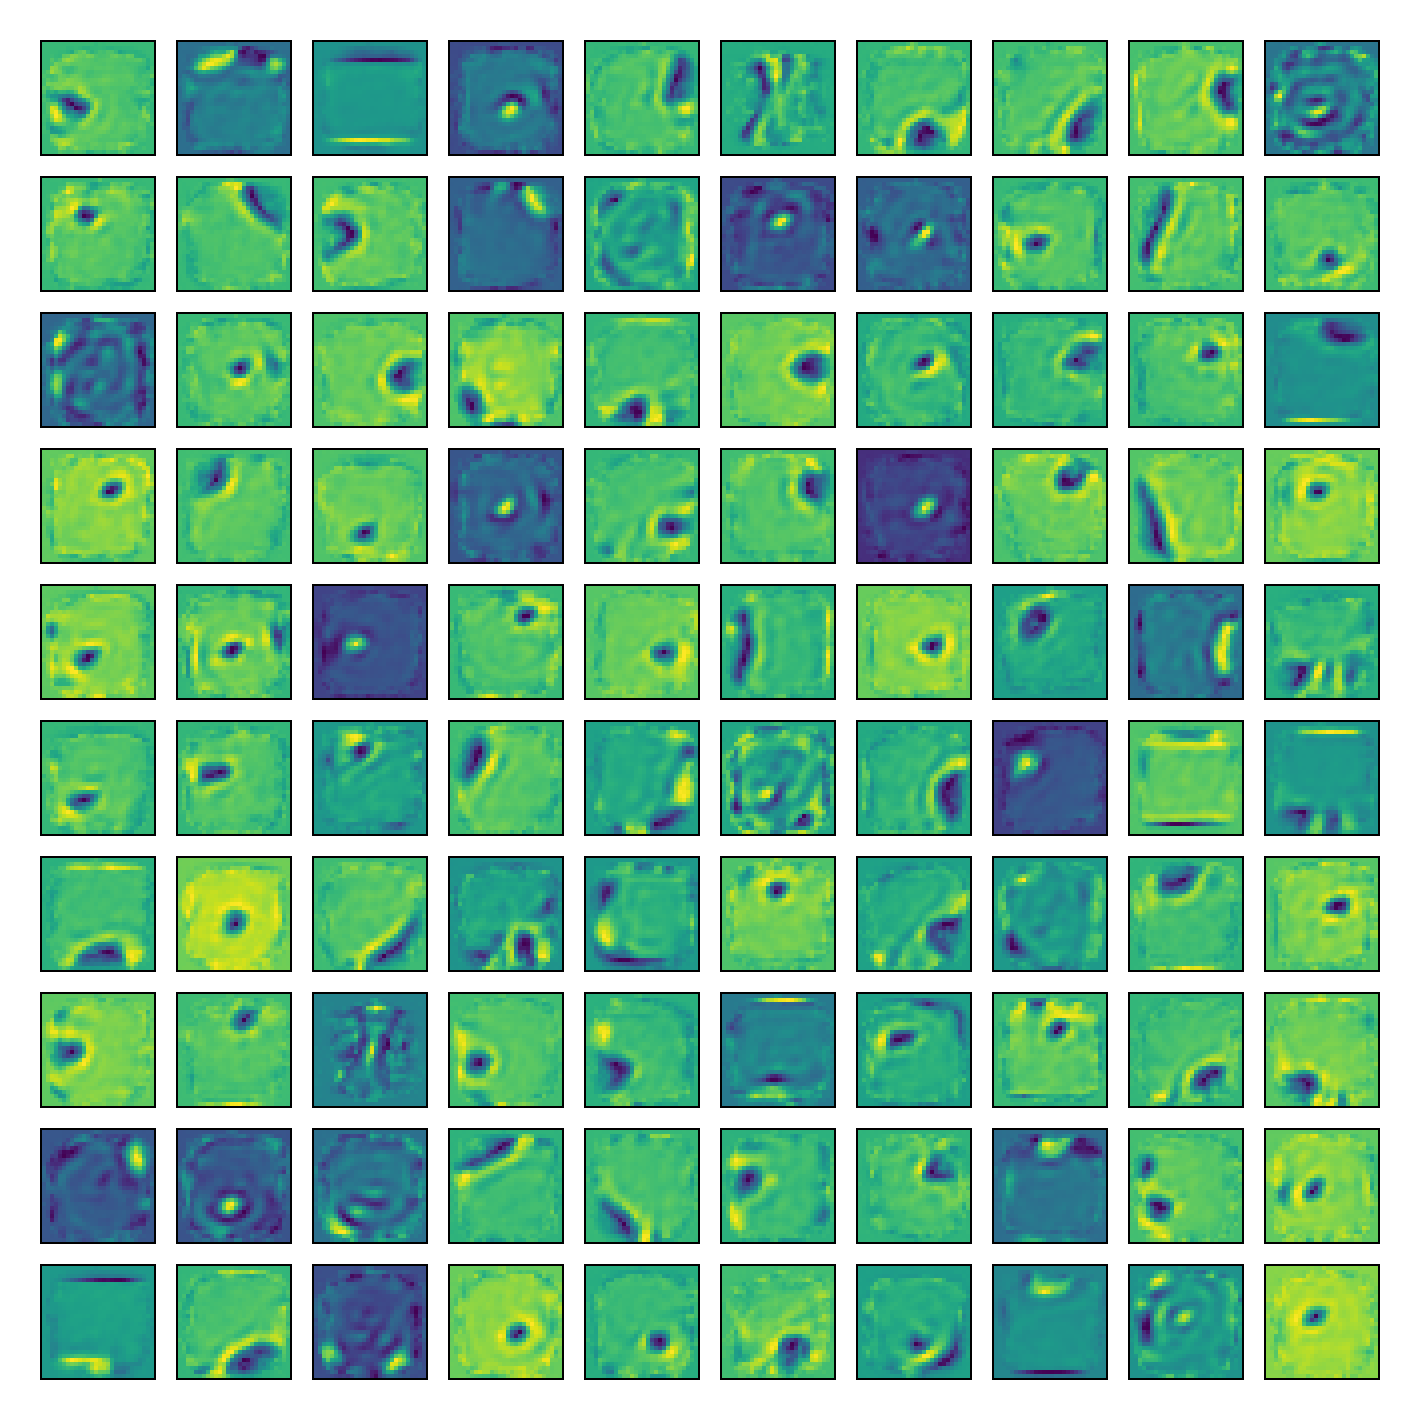
\includegraphics[width=\linewidth]{pictures/neuron_activations}
\end{center}
\end{column}
\end{columns}
\end{frame}

\begin{frame}[fragile]{Experiments}
j
\end{frame}

\end{document}